% !TEX encoding = UTF-8
% !TEX TS-program = pdflatex
% !TEX root = ../tesi.tex

%**************************************************************
\chapter{Progettazione}
\label{cap:progettazione}
%**************************************************************

In questo capitolo verrà descritta la progettazione dell'intero prodotto, in particolare verranno chiariti i seguenti argomenti:
\begin{itemize}
	\item progettazione delle classi che definiscono lo stato dell'applicazione;
	\item la gestione dello stato dell'applicazione;
	\item progettazione del parser json e dell'adapter per trasformare le informazioni ottenute dall'api nelle classi che definiscono lo stato dell'applicazione;
	\item la gestione del caricamento parziale;
	\item descrizione e progettazione dei componenti grafici.
\end{itemize}

\section{Entità dello stato}
Per quanto riguarda lo stato dell'applicazione ho analizzato la struttura della tabella fornita dall'azienda e le funzionalità richieste. L'idea alla base della struttura dello stato era quella di avere una struttura dati semplice da iterare in modo da avere funzioni di renderizzazione concise e facili da manutenere. Dalla struttura della tabella pivot e dalla descrizione delle sue funzionalità ho ricavato le seguenti strutture dati:
\paragraph*{data class DimensionsNode}- rappresenta una cella d'intestazione, deve contenere:
\begin{itemize}
	\item \verb|id|: codice della cella;
	\item \verb|label|: testo da renderizzare;
	\item \verb|level|: indica a che dimensione dell'intestazione appartiene la cella;
	\item \verb|childDepth|: indica la profondità della cella in una gerarchia ad albero;
	\item \verb|path|: codice identificativo della cella costituito da una lista di \verb|id| che rappresenta la gerarchia di una cella;
	\item \verb|actionType|: indica il tipo dell'azione che bisogna eseguire, esso verrà indicato con una classe di tipo: \verb|enum class NodeActionType|;
	\item \verb|isChild|: indica se la cella è un figlio di un'altra cella.
\end{itemize}

\paragraph*{data class BodyCells}- rappresenta una cella dei dati, deve contenere:
\begin{itemize}
	\item \verb|value|: indica il dato;
	\item \verb|cPath|: indica l'insieme dei codici delle dimensioni delle colonne a cui appartiene il dato;
	\item \verb|rPath|: indica l'insieme dei codici delle dimensioni delle righe a cui appartiene il dato.
\end{itemize}	

\paragraph*{data class HeaderAction}- rappresenta un tipo di azione, deve contenere:
\begin{itemize}
	\item \verb|actionType|:  indica il tipo dell'azione che bisogna eseguire, esso verrà indicato con una classe di tipo: \verb|enum class NodeActionType|;
	\item \verb|dim|: indica la dimensione su cui applicare l'azione;
	\item \verb|depth|: indica la profondità all'interno della dimensione su cui applicare l'azione.
\end{itemize}

\paragraph*{enum class NodeActionType}- rappresenta un tipo di azione:
\begin{itemize}
	\item \verb|EXPAND|:  indica che la cella può espandere per mostrare i suoi figli;
	\item \verb|COLLAPSE|: indica che la cella può nascondere i suoi figli;
	\item \verb|NULL|: indica che la cella non ha un'azione.
\end{itemize}

Quindi per rappresentare l'intero stato della tabella ho definito un ultimo \verb|data class|:
\paragraph*{data class TableState}
\begin{itemize}
	\item \verb|rows|: matrice di DimensionsNode, rappresenta le dimensioni delle righe;
	\item \verb|cols|: matrice di DimensionsNode, rappresenta le dimensioni delle colonne;
	\item \verb|cells|: matrice di BodyCells, rappresenta le celle contente i dati della tabella;
	\item \verb|rowActions|: matrice di HeaderAction, rappresenta le azioni disponibili per le dimensioni delle righe;
	\item \verb|colActions|:  matrice di HeaderAction, rappresenta le azioni disponibili per le dimensioni delle colonne.
\end{itemize}

\section{Gestione dello stato}
In questa sezione verrà descritto il ragionamento e il modo in cui è avvenuta la progettazione degli elementi che si occuperanno di gestire lo stato dell'applicazione.

\subsection{Dataflow dell'applicazione}
Un aspetto che è stato molto discusso dal team di sviluppo riguarda il \emph{dataflow}\glosp dell'applicazione. Durante la prima settimana del tirocinio, oltre allo studio delle tecnologie, si è pensato a come verrà gestito lo stato dell'applicazione e in particolare delle possibili soluzioni per garantirne la scalabilità. Verrà descritto il dataflow fornito da React e Redux, infine verrà identificato quello adottato nell'ambito del progetto.

\subsubsection*{React}
React è una libreria per realizzare interfacce utente che utilizza un \emph{dataflow} unidirezionale. Questo perchè ogni componente può avere uno stato locale accessibile solo da se stesso e può passare informazioni ai suoi componenti figli mediante le \emph{props}\glo. Il risultato è uno stato che dipende dalla gerarchia di componenti grafici. \\
Questo dataflow è molto semplice però presenta alcune limitazioni per quanto riguarda la scalabilità. Per avere uno stato unico di tutta l'applicazione bisognerebbe dare la responsabilità ad un componente grafico di gestirlo e passarlo mediante le sue \emph{props}. L'architettura che ne deriva, nel caso di applicazioni complesse con molti componenti, è limitata, difficile da manutenere e poco scalabile. \\
Tuttavia questo semplice dataflow ha il vantaggio che per famiglie di componenti piccole i cambiamenti di stato locale e i passaggi di informazioni mediante le \emph{props} sono molto veloci e semplici.

\subsubsection*{Redux}
Per garantire scalabilità e facilità nella gestione dello stato dell'applicazione abbiamo discusso riguardo l'utilizzo di Redux. Essa offre un dataflow unidirezionale dove lo stato è gestito in una struttura di Redux chiamata \emph{store}. Questa struttura esterna ai componenti grafici rende la gestione dello stato dell'applicazione più prevedibile e manutenibile. Redux si basa su tre principi:
\begin{itemize}
	\item lo stato è l'unica fonte di verità;
	\item lo stato non è modificabile direttamente;
	\item le modifiche avvengono medianti \emph{funzioni pure}\glosp che creano un nuovo stato per evitare \emph{side effects}\glo.
\end{itemize}
\noindent
Gli elementi dell'architettura di Redux sono i seguenti:
\begin{itemize}
	\item \textbf{Actions}: oggetti che rappresentano un azione che innesca un update dello stato;
	\item \textbf{Reducers}: \emph{funzioni pure} che hanno come parametro un Actions e si occupano di modificare lo stato;
	\item \textbf{Store}: lo Store è un'interfaccia che contiene lo stato dell'applicazione e fornisce funzioni per leggere, modificare e registrare \emph{listeners}\glosp allo stato.
\end{itemize}
\noindent

\subsection{Soluzione}
La soluzione adottata è stata quella di usare sia React che Redux. React è stato usato per gestire solo gli aggiornamenti visivi dell'applicazione, mentre Redux per gestire lo stato completo dell'applicazione. Il dataflow del prodotto è quindi il seguente:
\begin{enumerate}
	\item se l'utente esegue una azione che implica un cambiamento dello stato verrà mandata allo Store una Action;
	\item lo Store si occuperà di chiamare un Reducer in modo da ricevere lo stato successivo;
	\item lo stato verrà aggiornato e i cambiamenti saranno visibili a tutti i componenti React che sono registrati allo Store.
\end{enumerate}
Utilizzando questo dataflow lo stato dell'applicazione non dipende da un componente grafico perchè è esterno alla gerarchia dei componenti grafici. Quindi ogni componente React che ha bisogno di una frazione dei dati dello stato può semplicemente registrarsi allo Store per ricevere i dati.
\\
\\
Per applicare al meglio il dataflow precedentemente descritto ho progettato i componenti di Redux nel seguente modo. Per prima cosa ho suddiviso lo stato dell'applicazione in "Slice" cioè in pezzi di stato. In questo modo la struttura dello stato è modulare e scalabile dato che, se questa applicazione verrà ampliata in un futuro basterà aggiungere uno "slice" allo stato. Ogni slice deve essere strutturato nel seguente modo:
\begin{lstlisting}[caption={Esempio Slice}, label={lst:bodycells}, language=Kotlin]
object Slice {
	// Stato
	data class State( ... )
	
	// Thunk
	private val thunk = Thunk()
	fun funcThunk() : RThunk = thunk
	
	// Actions
	class Action(): RAction
	...
	
	// Reducer
	fun reducer(state: State = State(), action: RAction) : State { ... }
}
\end{lstlisting}

\subsubsection*{Stato}
In ogni slice deve essere definito un \verb|data class| che contiene tutte le informazioni che si vuole contenere nello "Slice". Per quanto riguarda la realizzazione della tabella pivot esso conterrà i seguenti campi dati:
\begin{itemize}
	\item \verb|isLoading|: valore booleano che indica se si stanno effettuando chiamate http o funzionalità asincrone;
	\item \verb|rows|: insieme di celle che rappresentano le dimensioni delle righe;
	\item \verb|cols|: insieme di celle che rappresentano le dimensioni delle colonne;
	\item \verb|cells|: insieme di celle che contengono i dati relativi alle dimensioni;
	\item \verb|rowActions|: insieme di possibili azioni eseguibili sulle dimensioni delle righe;
	\item \verb|colActions|: insieme di possibili azioni eseguibili sulle dimensioni delle colonne.
\end{itemize}

\subsubsection*{Actions}
Le actions sono definiti come delle classi di tipo \verb|RAction| che vengono usati per innescare l'update dello stato. Solitamente un'action si occuperà di modificare solo un campo dato dello stato. Quindi dalla mia precedente progettazione dello stato ho individuato cinque Actions:
\begin{itemize}
	\item \verb|class UpdateRows(): RAction|;
	\item \verb|class SetIsLoading(): RAction|;
	\item \verb|class UpdateCols(): RAction|;
	\item \verb|class UpdateCells(): RAction|;
	\item \verb|class UpdateRowActions(): RAction|;
	\item \verb|class UpdateColActions(): RAction|.
\end{itemize}

\subsubsection*{Thunk}
Nell'ambito di questo progetto i cambiamenti dello stato devono essere gestiti in modo asincrono, in quanto viene fornita una API di supporto. Dato che i cambiamenti allo stato innescati dalle Actions possono essere solo sincroni ho utilizzato un \emph{middleware} di Redux che fornisce le stesse funzionalità di un Actions ma ne espande l'utilità permettendo operazioni asincrone, questa interfaccia è definita come \verb|thunk|.
I \emph{thunk} sono usati per effettuare operazioni asincrone complesse, l'interfaccia dei Thunk purtroppo non era presente nell'implementazione di Redux di kotlin quindi ho realizzato una semplice interfaccia che implementa le funzionalità dei thunk.
\begin{lstlisting}[caption={Interfaccia Thunk}, label={lst:bodycells}, language=Kotlin]
interface RThunk : RAction {
	operator fun invoke(
	dispatch: (RAction) -> WrapperAction,
	getState: () -> AppState
	) : WrapperAction
}

fun rThunk() =
applyMiddleware<AppState, RAction, WrapperAction, RAction, WrapperAction>(
{ store ->
	{ next ->
		{ action ->
			if (action is RThunk)
			  action(store::dispatch, store::getState)
			else
			  next(action)
		}
	}
}
)

val nullAction = js {}.unsafeCast<WrapperAction>()
\end{lstlisting}

\subsubsection*{Reducer}
Un \emph{reducer} è una \emph{funzione pura} che riceve come argomento un \verb|RAction| e ritorna una copia dello stato modificato. In kotlin il modo per realizzare una funzione reducer è realizzare una struttura switch (in kotlin corrisponde ad una struttura when) dove vengono definiti tanti casi quanto sono le actions disponibili che vogliono essere utilizzate. Per le actions definite precedentemente:
\begin{lstlisting}[caption={Interfaccia Thunk}, label={lst:bodycells}, language=Kotlin]
fun reducer(state: State = State(), action: RAction) : State {
  return when (action) {
    is UpdateRows -> state.copy(...)
    is SetIsLoading -> state.copy(...)
    is UpdateCols -> state.copy(...)
    is UpdateCells -> state.copy(...)
    is UpdateRowActions -> state.copy(...)
    is UpdateColActions -> state.copy(...)
    else -> state
  }
}
\end{lstlisting}


\section{Parser e adapter}
Per quanto riguarda la progettazione del parser json per l'api ho per prima cosa definito i passaggi necessari per ottenere i dati dall'API di Gruppo4. Ho individuato la necessità di due funzioni \verb|fetch| e \verb|sendAction|, la prima per richiedere i dati iniziali e la seconda per ottenere nuovi dati in seguito all'azione passata per argomento a \verb|sendAction|. \\
Per quanto riguarda il parser del json ho studiato la struttura del json ritornato dall'API in modo da identificare tutte le data class \verb|@Serializable| che mi permetteranno di mappare il json in data class. La struttura del json è la seguente:
\begin{lstlisting}[caption={Struttura JSON API}, label={lst:bodycells}, language=json]
{
	"Rows": {
		"Paths": [
		["_all", "_all", ...], [ ... ]
		],
		"Actions": [
		{ "Action": "C", "Dim": 1, "Depth": 0 }, { ... }
		],
		"Tree": [
		{
			"Code": "_all",
			"Label": "All",
			"SubDim": [
			{
				"Code": "_all",
				"Label": "All",
				"SubDim": null,
				"Children": null
			}
			]  
		}
		]
	}
	"Cols": // stessa struttura di "Rows"
	"Cells": [
	  [51515, 2315, 747, 22],
	  [ ... ]
	],
	"Filters": [
	  {
	    "Filtered": false,
	    "ActiveFilters": ["f1", "f2", "f3"],
	    "Type": "list",
	    "Name": "associazioni_provincia",
	    "Label": "Associazioni per provincia"
	  }
	]
}
\end{lstlisting}
Da questa struttura ho identificato le seguenti \verb|data class @Serializable|:
\begin{itemize}
	\item \verb|Gruppo4Json|: rappresenta la struttura generale del json;
	\item \verb|Gruppo4Data|: rappresenta la struttura dei campi dati "Rows" e "Cols";
	\item \verb|Gruppo4Filter|: rappresenta la struttura contenuta nel campo dati "Filters";
	\item \verb|Gruppo4Actions|: rappresenta la struttura contenuta nel campo dati "Actions" all'interno di "Rows" e "Cols";
	\item \verb|Gruppo4Node|: rappresenta la struttura contenuta nel campo dati "Tree" all'interno di "Rows" e "Cols" e corrisponde ad un nodo della struttura ad albero.
\end{itemize}
\noindent
Per quanto riguarda la progettazione dell'adapter ho analizzato le data class ottenibili dal JSON e le data class definite nello stato. Da questa analisi ho individuato le seguenti funzioni da realizzare:
\begin{itemize}
	\item \verb|fun convertListOfGruppo4Node()|:
	\begin{itemize}
		\item si occuperà di convertire una lista di \verb|Gruppo4Node| in \verb|DimensionsNode|;
	\end{itemize}

	\item \verb|fun convertTree()|:
	\begin{itemize}
		\item si occuperà di convertire la struttura ad albero in una struttura più semplice da iterare;
	\end{itemize}
	
	\item \verb|fun convertListOfGruppo4Actions()|:
	\begin{itemize}
		\item si occuperà di convertire una lista di \verb|Gruppo4Actions| in \verb|HeaderAction|;
	\end{itemize}

	\item \verb|fun convertCells()|:
	\begin{itemize}
		\item si occuperà di unire i dati definiti nel campo dati "Cells" con i "Path" in modo da ottenere una matrice di \verb|BodyCells|.
	\end{itemize}
\end{itemize}

\section{Gestione del caricamento parziale}
Per quanto riguarda il caricamento parziale della tabella, l'azienda mi ha richiesto di realizzarlo sotto due aspetti. Il primo riguarda il caricamento parziale di informazioni quando si "apre" una cella d'intestazione delle dimensioni. Il secondo invece riguarda il caricamento parziale durante lo scroll di un utente.

\subsection*{Caricamento parziale di un nodo}
La struttura della tabella viene fornita dall'API sotto forma di struttura ad albero. Per realizzare il caricamento parziale di un nodo ho pensato di mantenere nello stato una copia di questa struttura. In questo modo quando viene aperto o chiuso un nodo di una dimensione viene sostituito nella struttura ad albero e infine viene trasformato nella struttura semplice utilizzata per la renderizzazione mediante le funzioni adapter.

\subsection*{Caricamento parziale scroll}
Per quanto riguarda il caricamento parziale della tabella durante lo scroll di un utente l'azienda mi ha richiesto di realizzare un componente che si occuperà di chiamare l'API quando l'utente raggiunge un punto preciso della tabella.

\section{Componenti grafici}
Per quanto riguarda la progettazione dei componenti grafici l'azienda mi ha dato completa libertà per quanto riguarda la loro struttura. La progettazione di essi consiste nel loro mockup e la definizione degli stili grafici necessari. Questa prima immagine rappresenta il mockup iniziale da cui sono partito: \\
\begin{minipage}{\linewidth}
	\makebox[\linewidth] {
		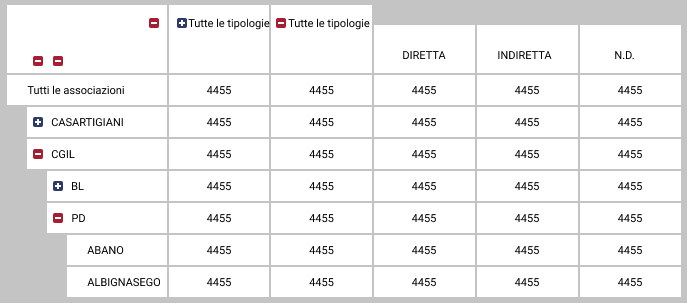
\includegraphics[scale=0.75]{./immagini/mockup-generale.png}
	}
\end{minipage}
\mbox{} \\
Da questo mockup generale ho individuato i seguenti componenti grafici. In particolare ho definito la loro gerarchia di composizione:
\begin{itemize}
	\item \verb|Table|
	\begin{itemize}
		\item \verb|TableActionUI|
		\item \verb|TableHeader|
		\begin{itemize}
			\item \verb|TableLabel|
		\end{itemize}
		\item \verb|TableSidebar|
		\begin{itemize}
			\item \verb|TableLabel|
		\end{itemize}
		\item \verb|TableBody|
	\end{itemize}
\end{itemize}

\noindent
Da questo mockup ho deciso in che modo organizzare questi componenti. In particolare ho suddiviso il componente \verb|Table| in quattro quadranti utilizzando \verb|css grid|. Ogni quadrante conterrà i singoli componenti. \\
Per quanto riguarda \verb|TableActionUI| ho pensato di suddividerlo in quattro quadranti in modo similare a \verb|Table| così da posizionare i pulsanti delle azioni in modo semplice.
In \verb|TableBody| ho definito la sua struttura come una tabella html.
Nel componente \verb|TableHeader| ho deciso di realizzare una tabella per ogni dimensione disponibile con una singola riga contenente un'insieme di \verb|TableLabel|.
Il componente \verb|TableSidebar| è simile a \verb|TableHeader|, quindi per ogni dimensione disponibile viene creata una tabella con una singola colonna contenente un'insieme di \verb|TableLabel|.
Infine per quanto riguarda il componente \verb|TableLabel| ho pensato di realizzarlo con un elemento \verb|<th>| con al suo interno un possibile pulsante per l'azione eseguibile e una etichetta, posizionati mediante l'uso di \verb|css flex|.








%**************************************************************
%\section{Introduzione al progetto}

%**************************************************************
%\section{Analisi preventiva dei rischi}

%Durante la fase di analisi iniziale sono stati individuati alcuni possibili rischi a cui si potrà andare incontro.
%Si è quindi proceduto a elaborare delle possibili soluzioni per far fronte a tali rischi.\\

%\begin{risk}{Performance del simulatore hardware}
%    \riskdescription{le performance del simulatore hardware e la comunicazione con questo potrebbero risultare lenti o non abbastanza buoni da causare il fallimento dei test}
%    \risksolution{coinvolgimento del responsabile a capo del progetto relativo il simulatore hardware}
 %   \label{risk:hardware-simulator} 
%\end{risk}

%**************************************************************
%\section{Requisiti e obiettivi}


%**************************************************************
%\section{Pianificazione}